\documentclass[10pt,a4paper,noendnumber=true]{scrartcl}
%german umlauts and localization
\usepackage[utf8]{inputenc} 
\usepackage[T1]{fontenc}
\usepackage[ngerman]{babel}
\usepackage[dvipsnames]{xcolor}
\usepackage{booktabs}
\usepackage{tabularx}

\usepackage{geometry}
\geometry{
	a4paper,
	total={170mm,257mm},
	left=20mm,
	top=20mm,
}

%figures etc.
\usepackage[pdftex]{graphicx}
\usepackage{standalone} %externalize files for faster compilation
\usepackage{float}

%mathematical symbols
\usepackage{latexsym} % special symbols 
\usepackage{amsmath,amssymb,amsthm}
\usepackage{textcomp} % supports the Text Companion fonts, which provide many text symbols (such as baht, bullet, copyright, musicalnote, onequarter, section, and yen)
%fonts:
%\usepackage{txfonts}  %supplies virtual text roman fonts using Adobe Times % needs to be loaded AFTER amsmath (because otherwise \iint is defined twice)
\usepackage{mathrsfs}  % for script-like fonts in math mode
\usepackage{nicefrac} % nice fracs in text

%\usepackage{libertine}
%\usepackage[libertine]{newtxmath}
%\usepackage[sc]{mathpazo}
%\linespread{1.05}

%tables
\usepackage{tabularx}

%units
\usepackage{siunitx}

%tikz
\usepackage{tikz}
\usepackage{tikzscale}
\usepackage{pgfplots} 
\usepackage{pgfgantt}
\usepackage{pdflscape}
\usepackage[european]{circuitikz}
\pgfplotsset{compat=newest} 
\pgfplotsset{plot coordinates/math parser=false}
\usetikzlibrary{shapes.geometric}
\usetikzlibrary{arrows.meta}
\usetikzlibrary{arrows}
\usetikzlibrary{shapes.symbols,shadows}

%bib stuff
\usepackage[draft = false]{hyperref}
\usepackage{csquotes}
\usepackage[backend=biber,style=ieee]{biblatex}
%\addbibresource{bib.bib}

% gescheiter Abstand nach paragraph
\newcommand{\properparagraph}[1]{\paragraph{\textcolor{Emerald}{#1}}\mbox{}\\}
\usepackage[parfill]{parskip}

% für die Auflistung von Vor- und Nachteilen in itemize-Umgebung
\newcommand\pro{\item[$+$]}
\newcommand\con{\item[$-$]}

%nice row vector
\newcommand{\rvect}[1]{\begin{bmatrix} #1 \end{bmatrix}}

%align multi pgfplots
\pgfplotsset{yticklabel style={text width=3em,align=right}}

\usetikzlibrary{external}
\tikzexternalize[optimize=false,prefix=tikz/] % activate!

\usepackage{subfig}
\renewcommand{\arraystretch}{1.6}

\title{Wohnheimanleitungen}
\subtitle{}
\author{Marvin Noll}
\date{10.10.2019}

\begin{document}
%\maketitle

\section{Kassenwart}
\subsection{Zusammenfassung}
Der Kassenwart\ldots
\begin{itemize}
	\item bezahlt Rechnungen der Wohnheim-Bars (N20/N24)
	\newline [ca. alle 2 Wochen]
	\item führt den Finanzordner (A4-Leitzordner) und das Kassenbuch (Excel-Worksheet)
	\newline [ca. alle 2 Wochen]
	\item sammelt überschüssige Einnahmen aus den Wohnheim-Bars (N20/N24) ein und bringt diese zur Bank
	\newline [ca. alle 6 Wochen]
	\item hat Kontovollmacht (tätigt Einkäufe in Online-Shops und alle sonstigen Aus-/Einzahlungen des Wohnheims)
	\newline [ca. einmal pro Semester]
\end{itemize}

\subsection{Aufnahme der Tätigkeit}
Bei Aufnahme der Tätigkeit als Kassenwart ist ein Besuch bei der Finanzabteilung des Studierendenwerks erforderlich. Bei diesem Termin wird eine Vollmacht für den Kassenwart über das Wohnheim-Konto beantragt (minimale Formalitäten: Name, Geburtsdatum, \ldots). Danach erhält dieser einen Online-Banking Zugriff und eine Girocard (ugs. "`EC-Karte"'). Da diese Vorgänge etwas Zeit brauchen (2\,\ldots\,4 Wochen), wäre es wünschenswert, wenn der Kassenwart die Tätigkeit für mindestens zwei Semester ausübt und vom Vorgänger eingearbeitet wird.

Der Termin bei der Wohnheim-Finanzabteilung kann z.B. per E-Mail (\texttt{fibu@sw-ka.de}, Betreff: \texttt{Aufnahme Tätigkeit Kassenwart Wohnheim Nancystrasse}) ausgemacht werden:
\begin{verbatim}
	Sehr geehrte Damen und Herren,
	in der letzten Vollversammlung des Wohnheims Nancystrasse 20 am xx.yy.zz
	wurde ich zum neuen Kassenwart gewählt.
	Nun benötige ich die Vollmacht für das Wohnheimkonto.
	Können Sie mir dazu einen Terminvorschlag senden?
	
	Mit freundlichen Grüßen
	Herbert Kasse
\end{verbatim}

\subsection{Bezahlen von Rechnungen der Wohnheim-Bars}
\begin{enumerate}
	\item Rechnungen werden von den Bar-Tutoren in die Briefkästen des Kassenwarts geworfen. 
	\\(Sollte dieser über den Zeitraum von einigen Tagen nicht im Wohnheim sein, kann die Rechnung auch zusätzlich per E-Mail verschickt werden.)
	
	\item Die Rechnung wird nun schnellstmöglich(1\,\ldots\,3 Tage) per Online-Überweisung beglichen.
	\begin{enumerate}
		\item Überwiesen wird mittels Online-Banking(\texttt{https://www.bw-bank.de/de/home.html})\\ \textit{Einloggen} $\rightarrow$ \textit{Online-Banking} $\rightarrow$ \textit{Banking} $\rightarrow$ \textit{Überweisung}
		
		\item Die Daten für die Überweisung werden der Rechnung entnommen und in die entsprechenden Felder eingetragen. Als Verwendungszweck wird beim Lieferanten "`Getränke Lagune"' die Schreibweise \texttt{Kunde: <Kunden-Nr.> Beleg: <Beleg-Nr.>} (steht beides auf der Rechnung; jede der zwei Bars hat eine eigene Kunden-Nr.) verwendet. (Beispiel siehe \autoref{fig:rechnungZahlen})
		
		\item Die für die Überweisung notwendige TAN wird (Stand 10/19) mit einem TAN-Generator erzeugt.
	\end{enumerate}

	\begin{figure}[H]
		\centering\setcounter{subfigure}{0}
		\subfloat[Rechnung in Papierform]{\includegraphics[width=0.3\textwidth]{img/kassenwart/rechnungExample.pdf}}\qquad
		\subfloat[Daten im Online-Banking]{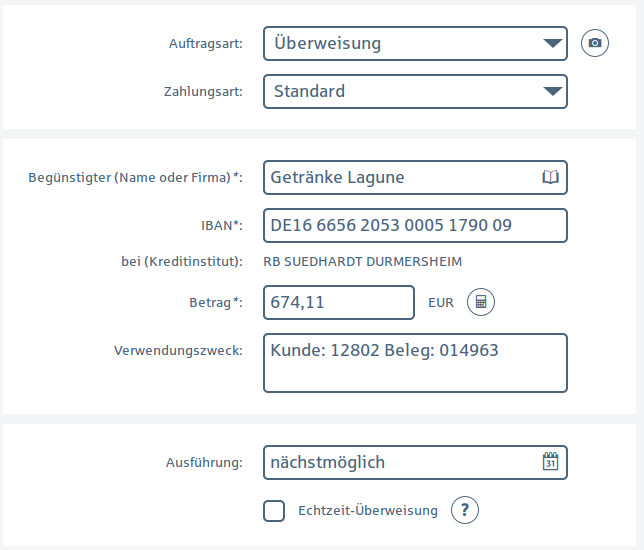
\includegraphics[width=0.4\textwidth]{img/kassenwart/onlineBanking.png}}
		\caption{Beispiel für das Zahlen einer Rechnung}\label{fig:rechnungZahlen}
	\end{figure}
	
	\item Die erfolgreiche Überweisung wird anschließend in das Kassenbuch eingetragen und die Rechnung in den Finanzordner abgeheftet.\\Dazu wird die Rechnung mit einer ID(\texttt{<Jahr>-<fortlaufende Nummer>}) mit Rotstift neben dem Adressfeld beschriftet.\footnote{also z.B. \texttt{19-12},\texttt{19-13},\,\ldots} Die ID wird auch im Kassenbuch vermerkt und dient dem leichteren Auffinden von Rechnungen.
	
	\item Nach Eintrag in das Kassenbuch wird der, vom Kassenbuch ermittelte (Soll-) Kontostand mit dem tatsächlichen Kontostand im Online-Banking verglichen:\\(\textit{Einloggen} $\rightarrow$ \textit{Online-Banking} $\rightarrow$ \textit{Umsätze} $\rightarrow$ \textit{Kontostand am \ldots} ablesen)
\end{enumerate}

\subsection{Führen des Finanzordners und des Kassenbuchs}
\begin{itemize}
	\item Der \textbf{Finanzordner} ist ein A4-"`Leitzhefter"' in dem alle Finanzdokumente des Wohnheims abgeheftet werden. Dies sind hauptsächlich Bar-Rechnungen und von der Bank per Post zugestellte Kontoauszüge. Aber auch Rechnungen für Ausgaben für den Fitnessraum, den Musikraum, das Winterfest, usw. werden hier abgelegt.
	
	\item Das \textbf{Kassenbuch} ist ein "`Excel"'-Worksheet\footnote{Freie Alternativen wie LibreOffice können auch genutzt werden.}. Hier werden alle Ein- und Ausgaben des Wohnheims vermerkt ($\approx$~20 Transaktionen pro Semester). Vom Worksheet werden Ein- und Ausgaben automatisch je nach Datum einem Semester zugeordnet. Zur Kontrolle wird der aktuelle (Soll-) Kontostand ermittelt.
	
	Die \texttt{.xlsx}-Datei ist auf einem USB-Stick gespeichert, der mit einer kleinen Kette im Finanzordner befestigt ist (und auch dort bleiben soll). Nach jeder Änderung wird die Datei unter neuem Namen abgespeichert, um Änderungen nachvollziehen zu können. Das Namensschema ist \texttt{Jahr\_Monat\_Tag\_nankasse.xlsx}\footnote{Wenn also eine Änderung z.B. am 01.12.19 eingetragen wird, ist der neue Dateiname \texttt{2019\_12\_01\_nankasse.xlsx}}.
\end{itemize}

\subsection{Einzahlung von Bargeld-Überschüssen der Wohnheim-Bars}
Bartutoren können dem Kassenwart aktiv Bargeld-Überschüsse übergeben, oder der Kassenwart kann diese bei den Bartutoren einfordern (vgl. Wohnheimordnung). Der Ablauf ist dann wie folgt:
\begin{enumerate}
	\item Der Kassenwart erhält die Bar-Überschüsse von einem Bar-Tutor. Bei der Übergabe zählen Kassenwart und Bar-Tutor die Geldscheine. Die Summe der Münzen soll zumindest auf Plausibilität geprüft werden.
	
	\item Der Kassenwart bewahrt das, ihm übergebene, Bargeld sicher auf und vermerkt die zugehörige Bar und den geschätzten Betrag (z.B. auf einem Notizzettel zusammen mit dem Geld)
	
	\item Das Geld sollte nun zeitnah bei der Bank eingezahlt werden.\\
	Die Filiale der BW-Bank in Karlsruhe liegt am Friedrichsplatz (Friedrichspl. 1-3, 76133 Karlsruhe). Erreichbar ist die Bank gut per Bahn(Haltestelle \textit{Herrenstrasse}), mit dem Fahrrad(vom \textit{Zirkel} in die \textit{Ritterstrasse} fahren) oder durch die Fußgängerzone zu Fuß. (vgl. \autoref{fig:bwbank})
	\begin{figure}[H]
		\centering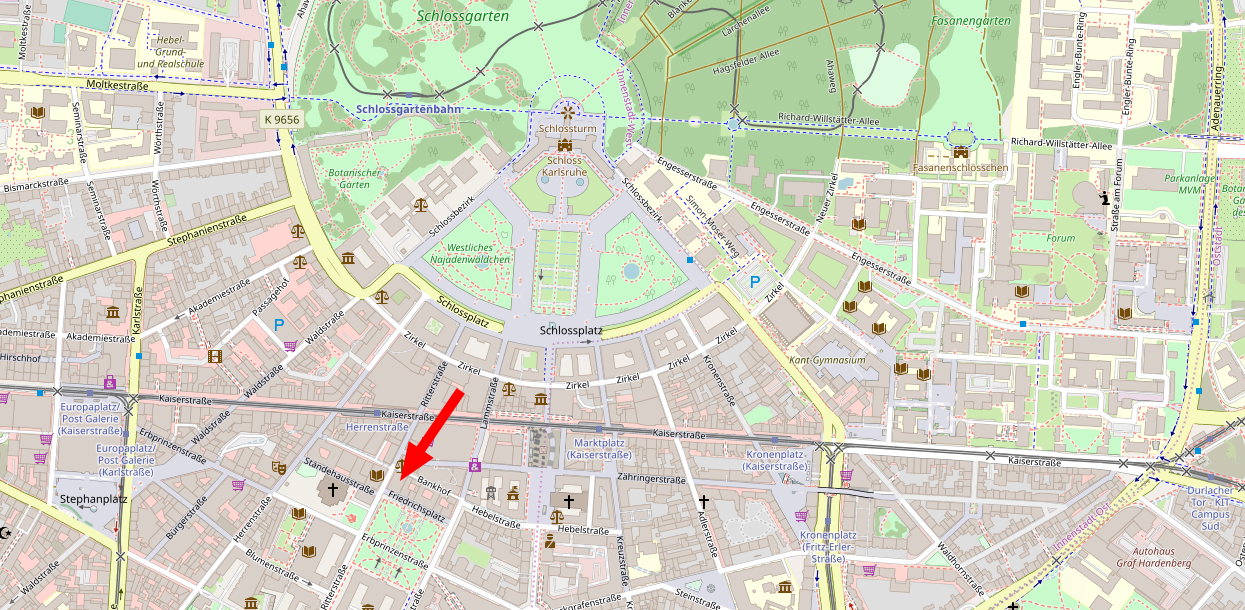
\includegraphics[width=0.6\textwidth]{img/kassenwart/bwbank.png}
		\caption{Lage BW-Bank (roter Pfeil)}\label{fig:bwbank}
	\end{figure}

	\item Die Einzahlung kann auf zwei Arten erfolgen:
	\begin{enumerate}
		\item \textbf{Nur Scheine:} Am einfachsten ist die Nutzung des Ein-/Auszahlungsautomaten im Eingangsbereich. Hierzu ist nur die EC-Karte erforderlich.\footnote{Manchmal werden Scheine zu unrecht als Falschgeld angezeigt. Diese werden dann eingezogen und später von den Bankmitarbeitern von Hand geprüft, womit das Thema dann eigentlich immer erledigt ist.}
		
		\item \textbf{Münzen} oder \textbf{Scheine+Münzen:} Sollen auch Münzen eingezahlt werden, erfolgt dies am Kassenschalter in der Filiale. Dazu holt man sich an einem der Pulte einen Einzahlungsbeleg\footnote{Tipp: Gleich mehrere "`unauffällig"' in die Tasche stecken und dann zu Hause in Ruhe ausfüllen.}. Dieser wird wie folgt beschriftet:
		\begin{itemize}
			\item Datum von heute
			\item Kontonummer(steht auf der EC-Karte)
			\item Anschrift(\texttt{Studierendenwerk Karlsruhe} reicht)
			\item Wenn mehrere Zahlungen an einem Tag vorgenommen werden, kann bei "`Angabe des Einzahlers"' z.B. die Bar(20 oder 24) vermerkt werden.
			\item Betrag und Unterschrift \textbf{NICHT} ausfüllen.
		\end{itemize}
		(Beispiel siehe \autoref{fig:einz})
		\begin{figure}[H]
			\centering\includegraphics[width=0.6\textwidth]{img/kassenwart/einzahlung.pdf}
			\caption{Ausgefüllter Einzahlungsbeleg vor Einzahlung}\label{fig:einz}
		\end{figure}
	
		\item Mit dem Geld und dem Einzahlungsbeleg zum Kassenschalter gehen:
		\begin{enumerate}
			\item \textbf{Kassenwart:} "`Guten Tag, ich möchte etwas einzahlen. Es sind auch Münzen dabei"'\\
			\textit{Scheine durch den Schlitz unter dem Glas schieben, Münz-Behältnis vorzeigen.}
			
			\item \textbf{Bankmitarbeiter:} "`Gerne. Stellen Sie den Behälter hier rein/Moment, ich komme raus."'
			
			\item \textbf{Kassenwart:} \textit{Behälter in die Box links stellen/warten.}
			
			\item \textbf{Bankmitarbeiter:} \textit{Zählt Münzen maschinell im Nebenraum, kommt mit Behälter und Ausdruck der Maschine zurück.} "`Das waren \ldots Euro."' \textit{Zählt die Scheine und zeigt das Ergebnis.}
			
			\item \textbf{Kassenwart:} \textit{Mit den Augen rollen.} "`Könnten Sie mir das mit den Münzen zusammenrechnen, bitte?"'
			
			\item \textbf{Bankmitarbeiter:} \textit{Berechnet die Summe.}
			
			\item \textbf{Kassenwart:} \textit{Summe auf dem Einzahlungsbeleg eintragen und diesen unterschreiben. Dann auch unter dem Glas durchschieben.}
			
			\item \textbf{Bankmitarbeiter:} \textit{Unterschreibt und übergibt den Durchschlag.}
			
			\item \textbf{Kassenwart:} "`Vielen Dank und auf Wiedersehen."'
		\end{enumerate}
	\end{enumerate}	

	\item Die erfolgreiche Einzahlung wird im Kassenbuch vermerkt indem die Summe auf die Bars verteilt wird.
	
	\item Nach Eintrag in das Kassenbuch wird der, vom Kassenbuch ermittelte (Soll-) Kontostand mit dem tatsächlichen Kontostand im Online-Banking verglichen:\\(\textit{Einloggen} $\rightarrow$ \textit{Online-Banking} $\rightarrow$ \textit{Umsätze} $\rightarrow$ \textit{Kontostand am \ldots} ablesen)
\end{enumerate}

\subsection{Einkäufe in Online-Shops und sonstige Aus-/Einzahlungen}
Sonstige Ein- und Auszahlungen werden meist individuell mit dem Wohnheimsprecher abgeklärt, laufen aber im Prinzip gleich ab, wie oben beschrieben.

\end{document}

